\chapter{Results}
\label{sec:results}

\newcommand{\sZero}{\shortstack[l]{\texttt{S1}\\\mbox{Zero-shot}}}
\newcommand{\sControl}{\shortstack[l]{\texttt{S23}\\\mbox{No-instruction}}}
\newcommand{\sPolicy}{\shortstack[l]{\texttt{S24}\\\mbox{Policy-first}}}
\newcommand{\sLeast}{\shortstack[l]{\texttt{S25}\\\mbox{Least-to-most}}}
\newcommand{\sSkeleton}{\shortstack[l]{\texttt{S26}\\\mbox{Skeleton}}}

This chapter reports the Tesla EV graph-recovery results stored in
\path{results/tesla_ev_graph_recovery}. The primary numerical source is
\path{results/tesla_ev_graph_recovery/evaluation_matrix_tesla_ev_long.csv};
edge-level interpretation uses the per-cell JSON files,
\path{results/tesla_ev_graph_recovery/edges_kg.csv}, and
\path{results/tesla_ev_graph_recovery/consensus_tesla_ev.csv}. No additional
experiments are introduced.

\summarynote{Reading guide}{Higher precision, recall, F1, and Pearson
correlation are better. Lower SHD, FDR, Hamming distance, and Frobenius norm
are better. Because every validated JSON sidecar reports \texttt{n\_runs = 1},
the tables describe observed model-strategy outputs, not repeated-run
stability.}

\section{Evaluation Matrix Overview}

The primary result matrix contains ten rows: two models evaluated under five
prompt strategies on the Tesla Full EV use case. Table~\ref{tab:graph-results}
lists the complete metric set and should be read as a descriptive comparison,
because each row represents one validated model-strategy output. The strongest
observed row is
\texttt{deepseek-r1:8b} with
\strategy{Strategy_26_Skeleton_of_Thought}, which reaches precision 0.4444,
recall 0.6667, F1 score 0.5333, SHD 7, FDR 0.5556, Pearson correlation
0.4303, Hamming distance 0.1944, and Frobenius norm 2.6458.

\begin{table}[!htbp]
  \centering
  \scriptsize
  \setlength{\tabcolsep}{2.5pt}
  \renewcommand{\arraystretch}{1.10}
  \begin{tabularx}{\textwidth}{@{}L{25mm}L{34mm}rrrrrrrr@{}}
    \toprule
    Model & Strategy & Prec. & Rec. & F1 & SHD & FDR & Pearson & Hamm. & Frob. \\
    \midrule
    \texttt{deepseek-r1:8b} & \sZero & 0.0000 & 0.0000 & 0.0000 & 6 & 0.0000 & 0.0000 & 0.1667 & 2.4495 \\
    \texttt{deepseek-r1:8b} & \sControl & 0.3333 & 0.5000 & 0.4000 & 9 & 0.6667 & 0.2582 & 0.2500 & 3.0000 \\
    \texttt{deepseek-r1:8b} & \sPolicy & 0.0000 & 0.0000 & 0.0000 & 6 & 0.0000 & 0.0000 & 0.1667 & 2.4495 \\
    \texttt{deepseek-r1:8b} & \sLeast & 0.0000 & 0.0000 & 0.0000 & 6 & 0.0000 & 0.0000 & 0.1667 & 2.4495 \\
    \texttt{deepseek-r1:8b} & \sSkeleton & \textbf{0.4444} & \textbf{0.6667} & \textbf{0.5333} & 7 & 0.5556 & \textbf{0.4303} & 0.1944 & 2.6458 \\
    \addlinespace
    \texttt{llama3.1:8b} & \sZero & 0.3333 & 0.5000 & 0.4000 & 9 & 0.6667 & 0.2582 & 0.2500 & 3.0000 \\
    \texttt{llama3.1:8b} & \sControl & 0.2857 & 0.3333 & 0.3077 & 9 & 0.7143 & 0.1569 & 0.2500 & 3.0000 \\
    \texttt{llama3.1:8b} & \sPolicy & 0.1667 & 0.1667 & 0.1667 & 10 & 0.8333 & 0.0000 & 0.2778 & 3.1623 \\
    \texttt{llama3.1:8b} & \sLeast & 0.2222 & 0.3333 & 0.2667 & 11 & 0.7778 & 0.0861 & 0.3056 & 3.3166 \\
    \texttt{llama3.1:8b} & \sSkeleton & 0.2222 & 0.3333 & 0.2667 & 11 & 0.7778 & 0.0861 & 0.3056 & 3.3166 \\
    \bottomrule
  \end{tabularx}
  \caption{Complete Tesla EV graph-recovery evaluation matrix from the long-format evaluation CSV. Strategy labels are abbreviated for readability; values are copied without numerical modification.}
  \label{tab:graph-results}
\end{table}

\begin{figure}[p]
  \centering
  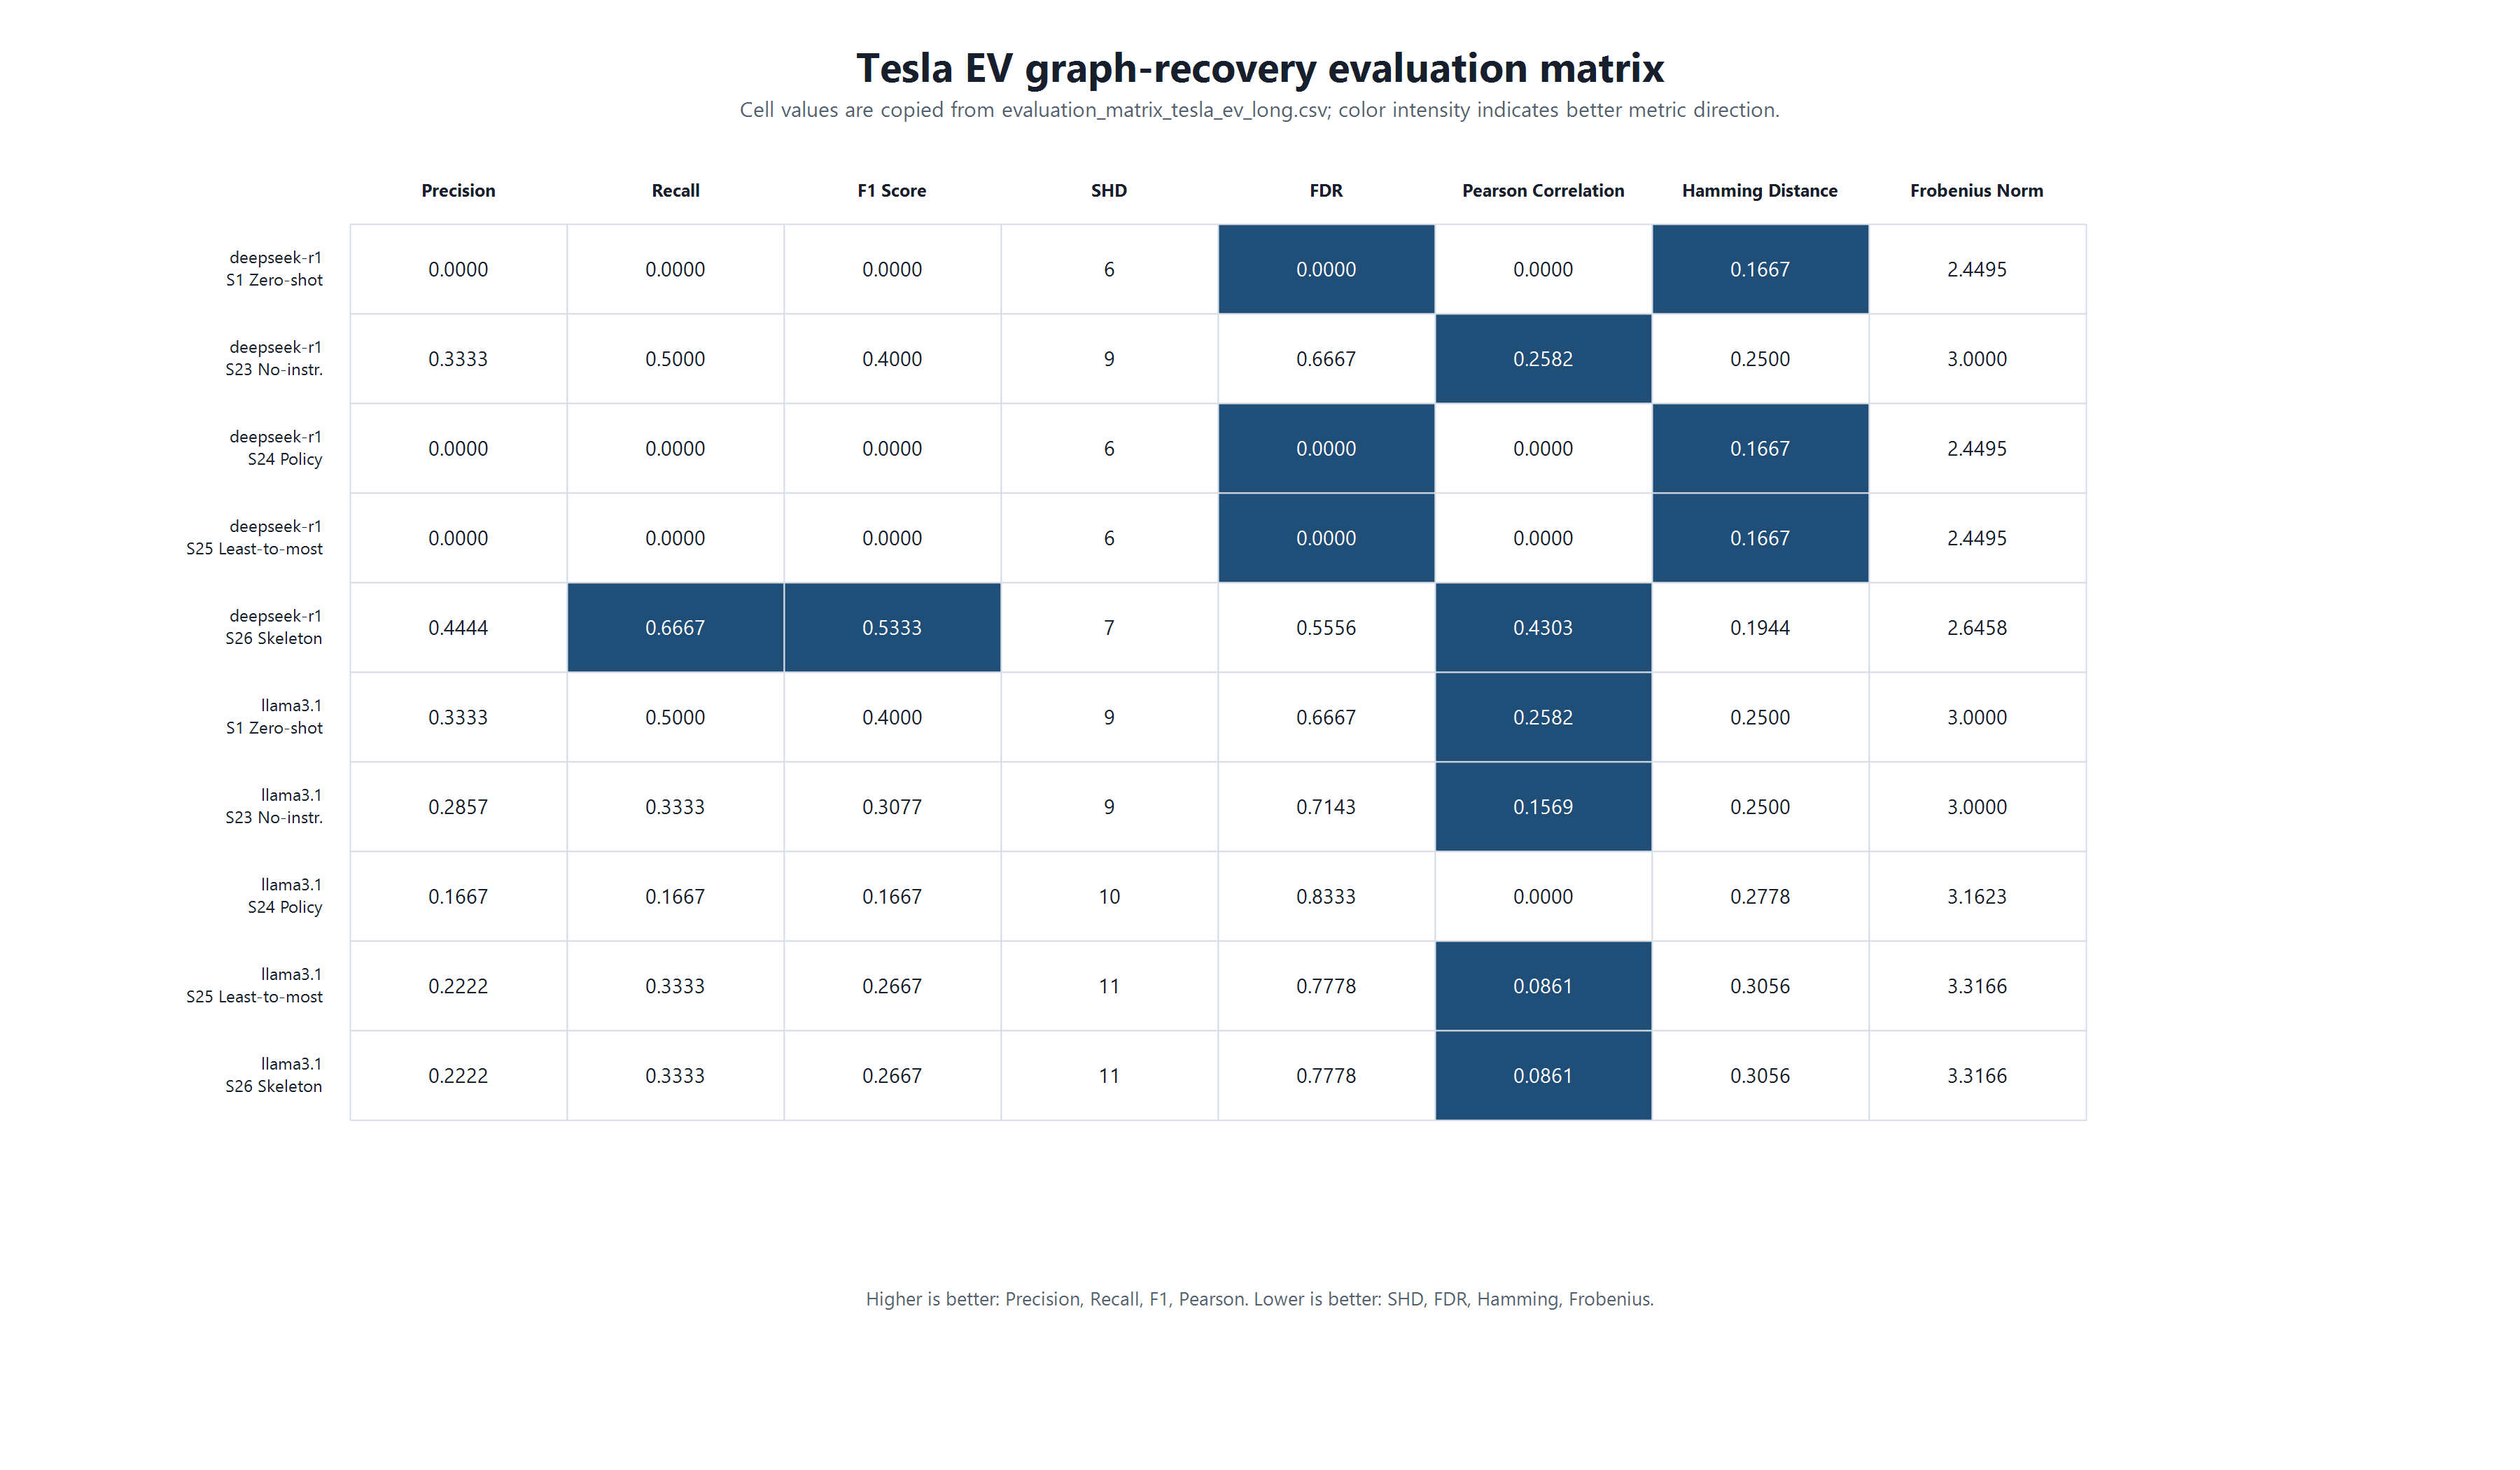
\includegraphics[width=\textwidth,height=0.62\textheight,keepaspectratio]{figures/evaluation_matrix_tesla_ev_heatmap.png}
  \caption{Evaluation matrix heatmap for the Tesla EV graph-recovery task. The visual summary complements Table~\ref{tab:graph-results} by showing how edge-recovery and structural-error metrics vary across model-strategy cells.}
  \label{fig:evaluation-matrix-heatmap}
\end{figure}

Figure~\ref{fig:evaluation-matrix-heatmap} makes the central pattern visible:
ranking is not monotonic with prompt complexity. The best row is a
decomposition-style strategy, yet several structured rows perform poorly.
DeepSeek with policy-first prompting and least-to-most prompting produces no
parseable predicted edges in the validated sidecars, yielding F1 score 0.0000.
Llama produces non-empty graphs in every evaluated strategy, but it often
overpredicts false edges.

\section{Model Comparison}

The two models show different failure profiles. Table~\ref{tab:model-average-results}
summarizes this contrast: averaged over the five prompt strategies, Llama has
higher mean F1 than DeepSeek, while DeepSeek has lower mean structural error.
This apparent tension is explained by empty outputs: three DeepSeek cells
predict no edges, which keeps SHD at 6 for those rows but also gives zero
recall and zero F1. Llama usually predicts edges, recovering more true
positives but also adding more false positives.

\begin{table}[!htbp]
  \centering
  \scriptsize
  \setlength{\tabcolsep}{3pt}
  \begin{tabular}{@{}lrrrrrr@{}}
    \toprule
    Model & Mean precision & Mean recall & Mean F1 & Mean SHD & Mean FDR & Mean Pearson \\
    \midrule
    \texttt{deepseek-r1:8b} & 0.1555 & 0.2333 & 0.1867 & 6.8000 & 0.2445 & 0.1377 \\
    \texttt{llama3.1:8b} & 0.2460 & 0.3333 & 0.2816 & 10.0000 & 0.7540 & 0.1175 \\
    \bottomrule
  \end{tabular}
  \caption{Model-level averages across the five evaluated strategies. The averages are descriptive because the experiment contains one output per model-strategy cell.}
  \label{tab:model-average-results}
\end{table}

DeepSeek is therefore not simply better or worse than Llama. It produces the
best single result under skeleton-of-thought prompting, but it also has three
zero-edge cells. Llama is more consistently non-empty but more prone to
spurious relationships, especially mileage-distance reversals and
energy-to-usage edges that are not in the ground truth.

\section{Strategy Comparison}

Table~\ref{tab:strategy-average-results} averages each strategy across both
models. Skeleton-of-thought has the highest mean F1 score, 0.4000, driven by
the strong DeepSeek skeleton result and the moderate Llama skeleton result.
The no-instruction control is second, with mean F1 0.3539. Policy-first
structured prompting is weakest by mean F1, 0.0834.

\begin{table}[!htbp]
  \centering
  \scriptsize
  \setlength{\tabcolsep}{3pt}
  \begin{tabular}{@{}lrrrrrr@{}}
    \toprule
    Strategy & Mean precision & Mean recall & Mean F1 & Mean SHD & Mean FDR & Mean Pearson \\
    \midrule
    \sSkeleton & 0.3333 & 0.5000 & 0.4000 & 9.0000 & 0.6667 & 0.2582 \\
    \sControl & 0.3095 & 0.4167 & 0.3539 & 9.0000 & 0.6905 & 0.2076 \\
    \sZero & 0.1667 & 0.2500 & 0.2000 & 7.5000 & 0.3334 & 0.1291 \\
    \sLeast & 0.1111 & 0.1667 & 0.1334 & 8.5000 & 0.3889 & 0.0431 \\
    \sPolicy & 0.0834 & 0.0834 & 0.0834 & 8.0000 & 0.4167 & 0.0000 \\
    \bottomrule
  \end{tabular}
  \caption{Strategy-level averages across DeepSeek and Llama3.1. Strategy labels use the same abbreviations as Table~\ref{tab:graph-results}; the ranking is descriptive and should not be read as a repeated-run result.}
  \label{tab:strategy-average-results}
\end{table}

\begin{figure}[p]
  \centering
  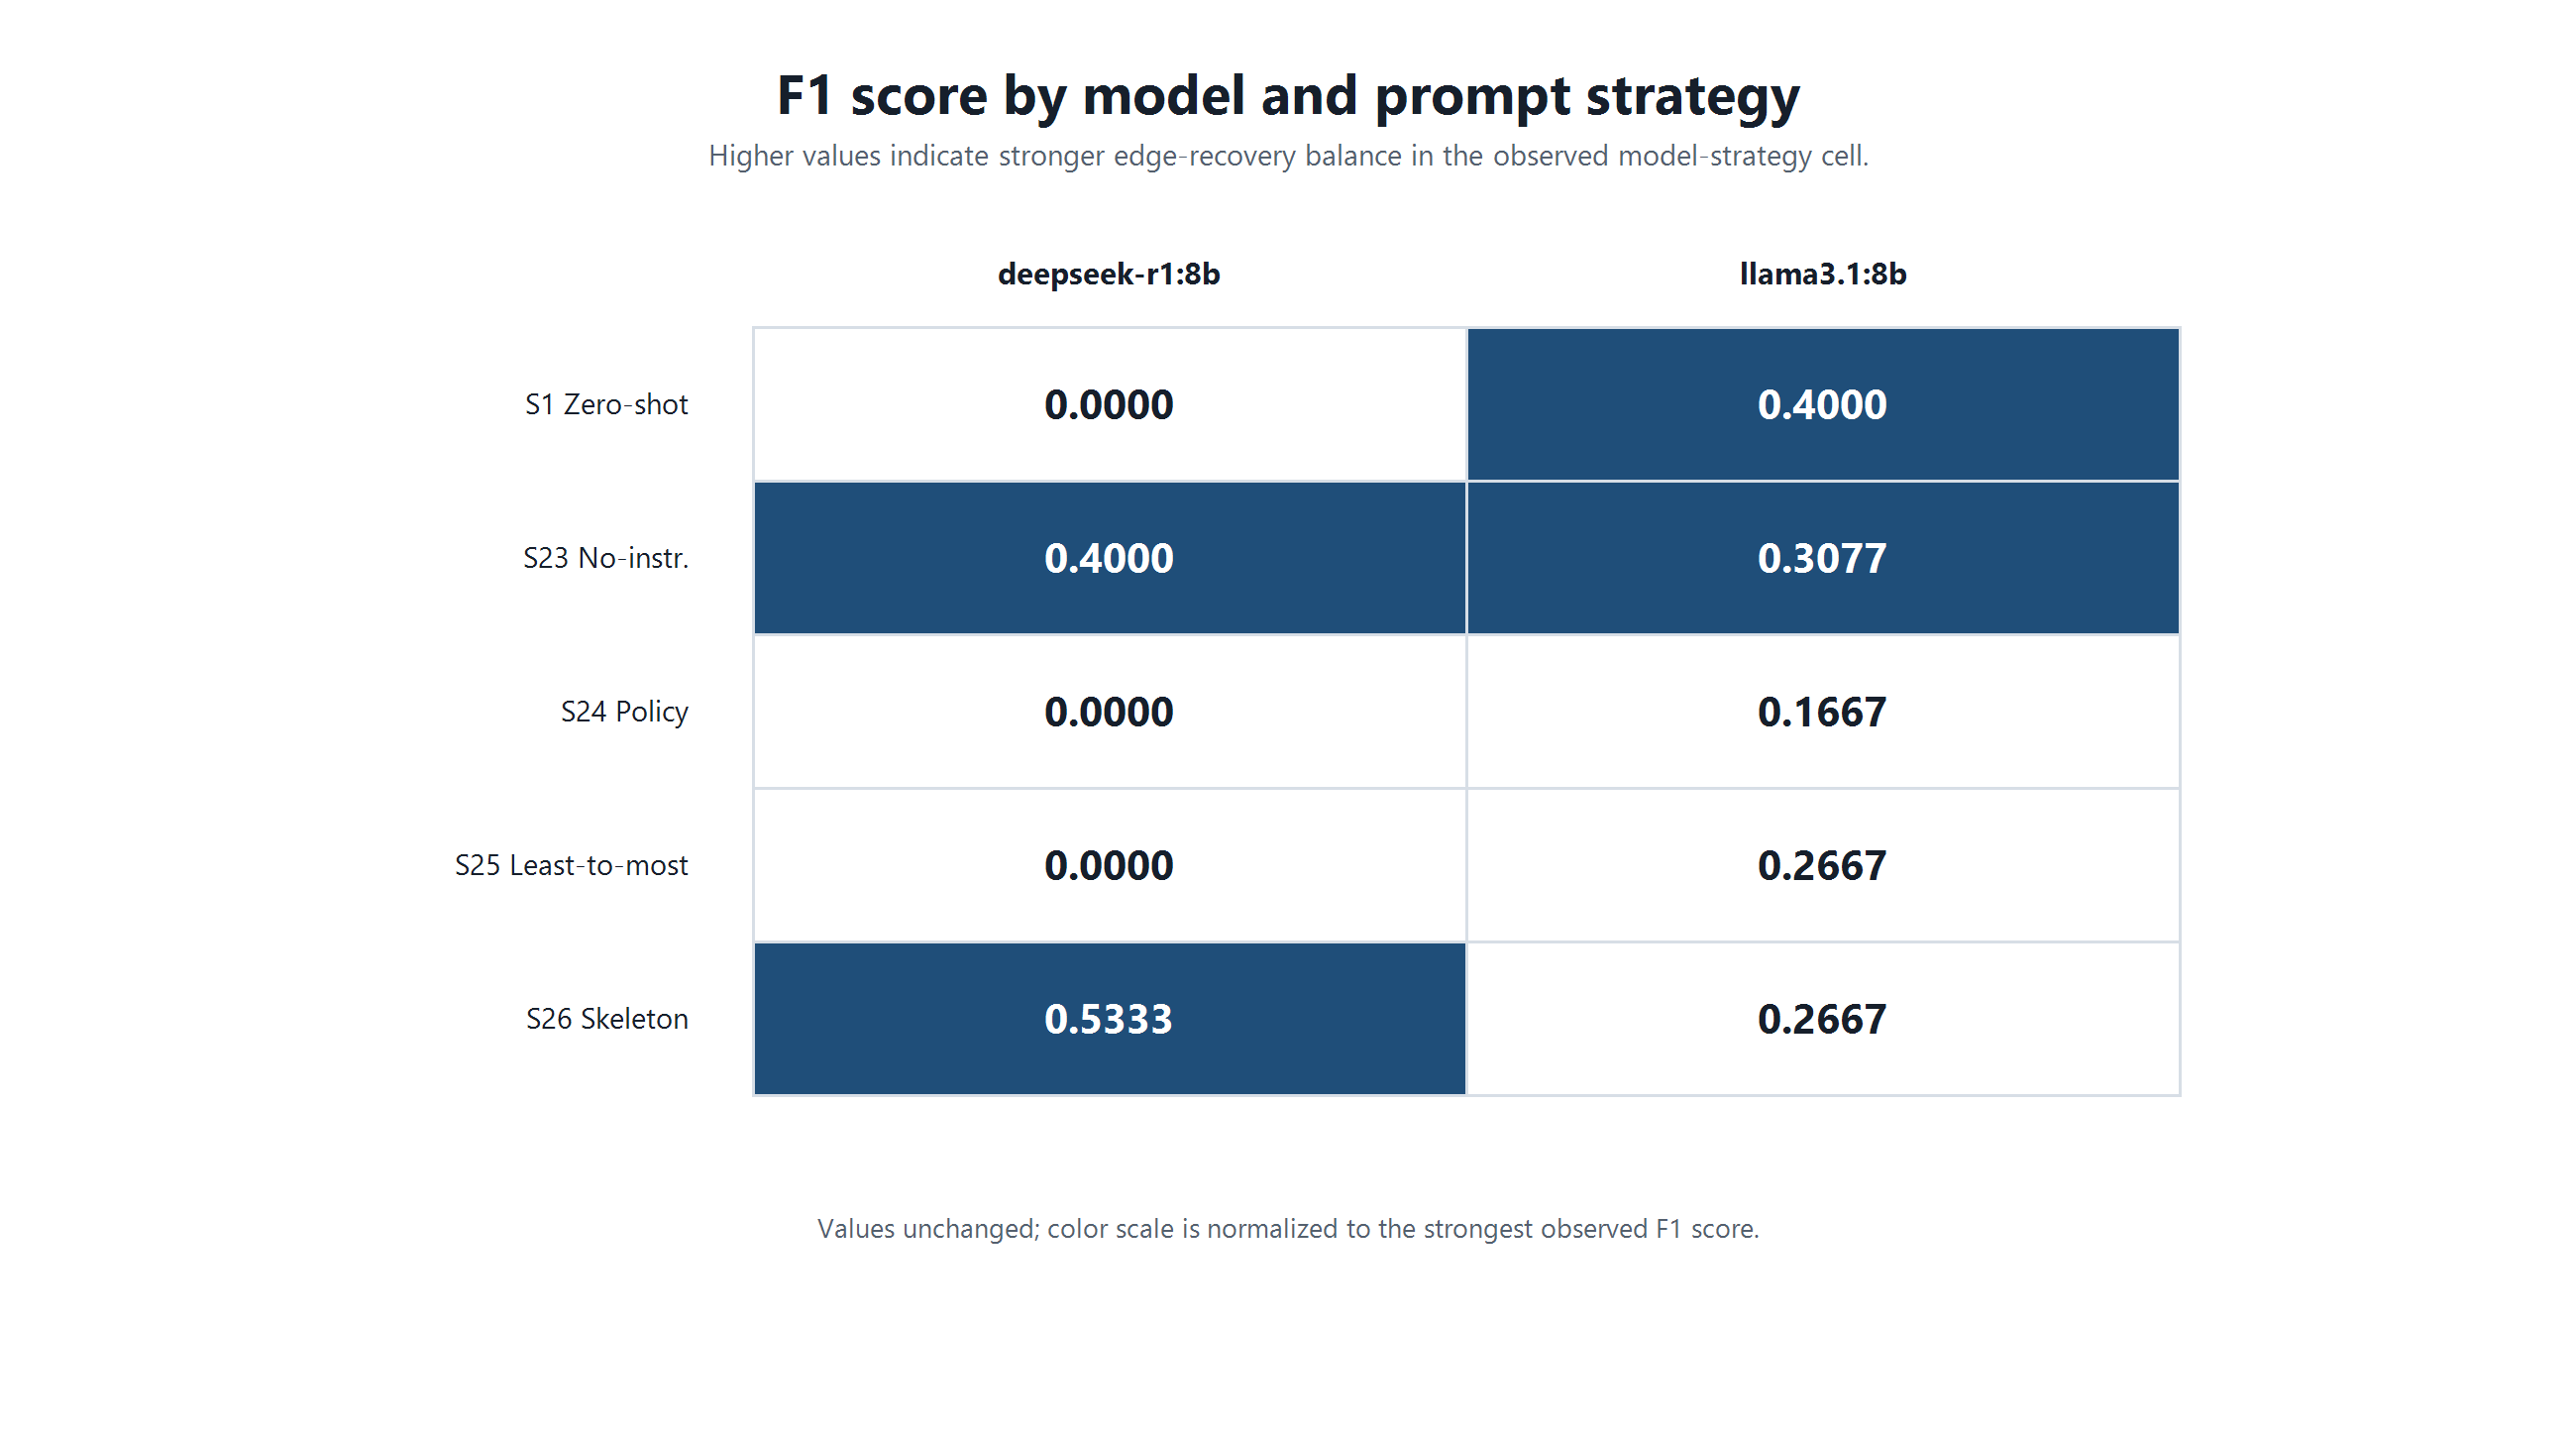
\includegraphics[width=\textwidth,height=0.58\textheight,keepaspectratio]{figures/f1_strategy_vs_model_tesla_ev.png}
  \caption{F1 heatmap by strategy and model. The strongest cell is DeepSeek with skeleton-of-thought prompting; the same figure also shows that the strategy effect differs by model.}
  \label{fig:f1-strategy-model}
\end{figure}

The decomposition evidence is therefore mixed but meaningful. As
Figure~\ref{fig:f1-strategy-model} shows, skeleton-of-thought is the best
strategy on average and gives the best overall cell. Least-to-most does not
show the same benefit: it produces an empty DeepSeek
output and a high-false-positive Llama output. The difference suggests that
decomposition is useful only when the decomposition structure matches the
model's output behavior and preserves the final edge-list contract.

\section{Edge-Level Analysis}

The best cell, DeepSeek with skeleton-of-thought, predicts nine edges. Four
are true positives and five are false positives. It recovers the
energy-to-range edge, the speed-to-distance edge, and the two driving-to-energy
edges. It misses \texttt{acceleration\_kmh2 -> speed\_kmh} and
\texttt{speed\_kmh -> mileage}. It also predicts false edges, including
\texttt{speed\_kmh -> acceleration\_kmh2},
\texttt{acceleration\_kmh2 -> distance\_m}, and
\texttt{distance\_m -> mileage}.

Table~\ref{tab:edge-level-results} summarizes the main edge-level patterns in
the representative cells used for interpretation.

\begin{table}[!htbp]
  \centering
  \scriptsize
  \setlength{\tabcolsep}{3pt}
  \renewcommand{\arraystretch}{1.12}
  \begin{tabularx}{\textwidth}{@{}L{31mm}rrrrY@{}}
    \toprule
    Model / strategy & Pred. & TP & FP & FN & Main edge-level pattern \\
    \midrule
    \shortstack[l]{\texttt{deepseek-r1:8b}\\\sSkeleton} & 9 & 4 & 5 & 2 & Best recovery; captures energy links and speed-to-distance, but reverses acceleration/speed and adds downstream energy/range edges. \\
    \shortstack[l]{\texttt{llama3.1:8b}\\\sZero} & 9 & 3 & 6 & 3 & Recovers three true edges but adds several reversed or energy-to-speed links. \\
    \shortstack[l]{\texttt{deepseek-r1:8b}\\\sControl} & 9 & 3 & 6 & 3 & Recovers three true edges but adds false links from \texttt{electricremaining} and a speed-to-acceleration reversal. \\
    \shortstack[l]{\texttt{llama3.1:8b}\\\sPolicy} & 6 & 1 & 5 & 5 & Retains only the energy-to-range ground-truth edge. \\
    \shortstack[l]{\texttt{deepseek-r1:8b}\\S1/S24/S25} & 0 & 0 & 0 & 6 & Empty raw outputs in the validated sidecars; no graph recovered. \\
    \bottomrule
  \end{tabularx}
  \caption{Edge-level interpretation of representative model-strategy cells. Counts are derived from per-cell JSON edge lists and the six-edge ground truth.}
  \label{tab:edge-level-results}
\end{table}

The most frequent false-positive pattern is direction reversal. The false edge
\texttt{speed\_kmh -> acceleration\_kmh2} appears in seven predicted edge
sets, while the ground truth contains the opposite direction
\texttt{acceleration\_kmh2 -> speed\_kmh}. Mileage and distance are also often
reversed: \texttt{mileage -> distance\_m} appears six times, and
\texttt{distance\_m -> mileage} appears five times, while the ground truth
contains \texttt{speed\_kmh -> mileage} and \texttt{speed\_kmh -> distance\_m}.

These errors are scientifically important. They show that the models often
identify semantically related feature pairs but fail to recover the evaluated
direction or the directness constraint. For fleet monitoring, that distinction
matters: a graph with plausible but reversed edges can mislead downstream
reasoning even if it appears domain-relevant.

\section{Consensus Graph}

The consensus file keeps edges that receive support from at least half of the
ten model-strategy cells. Five edges meet this threshold, shown in
Table~\ref{tab:consensus-results}. Only two of them are ground-truth edges.

\begin{table}[!htbp]
  \centering
  \small
  \setlength{\tabcolsep}{2pt}
  \begin{tabularx}{\textwidth}{@{}L{48mm}L{48mm}rrL{18mm}@{}}
    \toprule
    Source & Target & Votes & Support & Ground truth? \\
    \midrule
    \texttt{electricenergyremaining} & \texttt{electricremaining} & 7 & 0.7 & Yes \\
    \texttt{speed\_kmh} & \texttt{acceleration\_kmh2} & 7 & 0.7 & No \\
    \texttt{mileage} & \texttt{distance\_m} & 6 & 0.6 & No \\
    \texttt{acceleration\_kmh2} & \texttt{speed\_kmh} & 5 & 0.5 & Yes \\
    \texttt{distance\_m} & \texttt{mileage} & 5 & 0.5 & No \\
    \bottomrule
  \end{tabularx}
  \caption{Consensus edges from the supervisor-provided consensus CSV. Consensus identifies recurring model beliefs, but it does not guarantee correctness.}
  \label{tab:consensus-results}
\end{table}

The consensus graph therefore acts as an error-analysis tool rather than a
replacement for the ground truth. It highlights the robust
\texttt{electricenergyremaining -> electricremaining} relationship and the
\texttt{acceleration\_kmh2 -> speed\_kmh} relationship. It also amplifies
recurring mistakes: speed-to-acceleration and mileage-distance reversals are
popular enough to pass the consensus threshold.

\section{Summary of Findings}

The validated results support five findings:

\begin{itemize}
  \item skeleton-of-thought prompting with DeepSeek is the best single
  model-strategy cell by F1 score and Pearson correlation;
  \item Llama has higher average F1 across strategies, but also much higher
  average false discovery rate and structural error;
  \item DeepSeek is more brittle in this artifact set because three strategy
  cells contain empty raw outputs and zero predicted edges;
  \item prompt decomposition is not uniformly beneficial: skeleton-of-thought
  helps, while least-to-most does not improve the evaluated graph recovery;
  \item consensus edges reveal both stable true relationships and stable false
  beliefs, especially direction reversals.
\end{itemize}

These findings remain tied to the artifact set: one dataset, two models,
five active prompt strategies, and one validated output per model-strategy
cell.
